\documentclass[nobib]{tufte-handout}

\title{Tentamen i kombinatorik, 15 Mars 2023 $\cdot$ 1MA020}

\author[Vilhelm Agdur]{Vilhelm Agdur\thanks{Jag kommer besöka tentasalen för att svara på frågor cirka 15:30. Om ni behöver nå mig för frågor utanför den tiden kan ni nå mig på \href{mailto:vilhelm.agdur@math.uu.se}{\nolinkurl{vilhelm.agdur@math.uu.se}} eller per telefon på \texttt{072-373 32 90}.}}

\date{15 mars 2023}


%\geometry{showframe} % display margins for debugging page layout

\usepackage{graphicx} % allow embedded images
  \setkeys{Gin}{width=\linewidth,totalheight=\textheight,keepaspectratio}
  \graphicspath{{graphics/}} % set of paths to search for images
\usepackage{amsmath}  % extended mathematics
\usepackage{booktabs} % book-quality tables
\usepackage{units}    % non-stacked fractions and better unit spacing
\usepackage{multicol} % multiple column layout facilities
\usepackage{lipsum}   % filler text
\usepackage{fancyvrb} % extended verbatim environments
  \fvset{fontsize=\normalsize}% default font size for fancy-verbatim environments

\usepackage{color,soul} % Highlights for text


\include{mathcommands.extratex}
\setlength{\extrarowheight}{12pt}

\begin{document}

\definecolor{darkgreen}{rgb}{0.0627, 0.4588, 0.1451}

\maketitle% this prints the handout title, author, and date

\begin{abstract}
\noindent
Lycka till! {\vspace{0cm}
\includegraphics[height=0.08\textwidth]{graphics/burning-heart-emoji.png} 
\includegraphics[height=0.08\textwidth]{graphics/lily-emoji.png}}
\end{abstract}

\section{Fråga 1 (5 poäng)} % del 1
Låt, för varje $n$ och $k$ i $\N$, $f_{n,k}$ vara antalet etiketterade skogar på $n$ noder bestående av $k$ stycken träd.

\textbf{Delfråga a:} \emph{(2p)} Använd vad du vet om multinomialkoefficienter och Cayleys formel för att förklara varför
$$f_{n,k} = \frac{1}{k!}\sum_{\substack{n_1, n_2, \ldots, n_k\\ n_i \geq 1\\n_1 + n_2 + \ldots + n_k = n}} \binom{n}{n_1, n_2, \ldots, n_k}n_1^{n_1-2}n_2^{n_2-2}\ldots n_k^{n_k-2}.$$

\textbf{Delfråga b:} \emph{(3p)} Vi säger att ett etiketterat träd har \emph{ökande} etiketter ifall varje nod får en etikett som är större än sin förälder.

\begin{marginfigure}
  \centering
  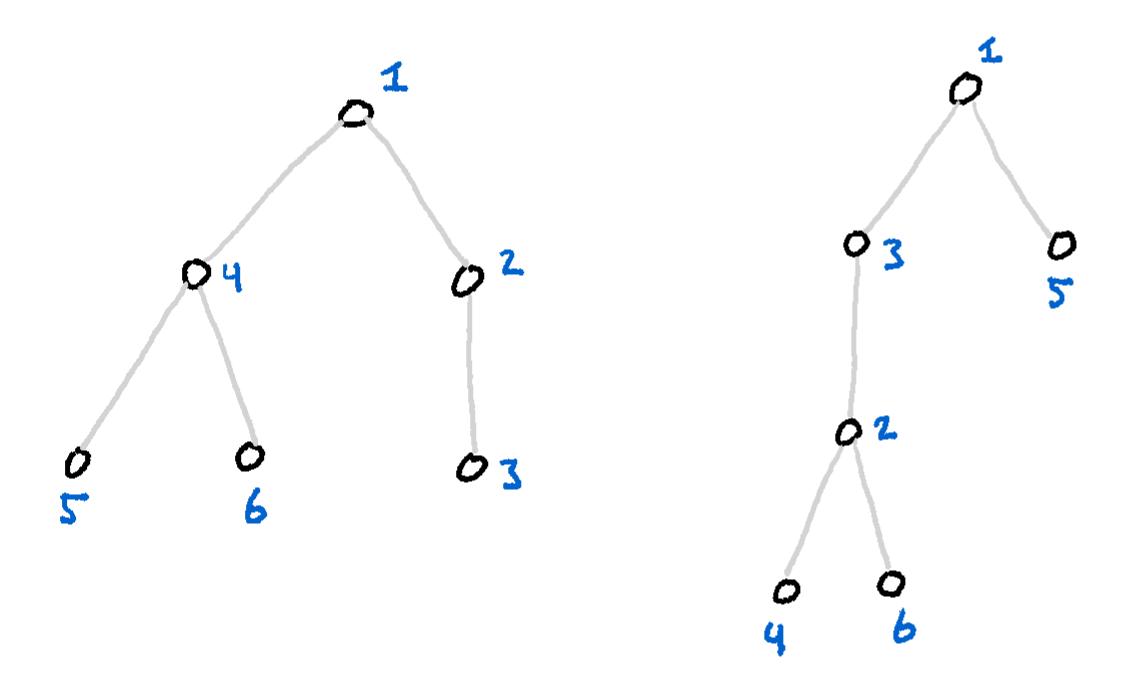
\includegraphics[width=\textwidth]{graphics/increasing_trees_figure.png}
  \caption{Två stycken etiketterade träd - det till vänster har en ökande etikettering, det till höger har det inte.}
\end{marginfigure}

Låt $t_{n,k}$ vara antalet etiketterade skogar på $n$ noder bestående av $k$ stycken träd, där etiketteringen är ökande. Ge ett kombinatoriskt bevis för att dessa ges av rekursionen
$$t_{n,k} = (n-1)t_{n-1,k} + t_{n-1, k-1}$$
med randvillkor
$$t_{n,n} = 1\, \forall\, n \geq 1,\quad t_{n,0} = 0\, \forall\, n \geq 1,\quad t_{n,k} = 0\text{ om }n < k.$$

\section{Fråga 2 (5 poäng)} % del 1

Vi ritade en tre-gånger-fyra-tabell av olika räkneproblem i kursen, som vi kallade för den tolvfaldiga vägen. I formelsamlingen ni fått med denna tenta finns den med -- men bara med formlerna, namnen på problemen är borttagna och namnen på rader och kolumner har ersatts med lorem ipsum.

\textbf{Delfråga a:} \emph{(2.5p)} Rita upp denna tabell med korrekta etiketter på rader och kolumner. För de celler i formelsamlingens tabell där formeln är \textcolor{red}{röd} ska du också skriva i namnet vi gett detta räkneproblem i din tabell.

\textbf{Delfråga b:} \emph{(2.5p)} Förklara, för alla problemen i första raden, det mellersta i andra raden, och det sista i tredje raden, varför det problemet hör hemma i den cellen. Du behöver inte bevisa att formeln för problemet stämmer, bara motivera varför problemet hör hemma i just den cellen -- alltså varför den kombinationen av rad och kolumn motsvarar det problemet.

\section{Fråga 3 (5 poäng)} % del 2

Betrakta ekvationen
$$x_1 + x_2 + x_3 + x_4 = n$$
där vi kräver att alla variablerna är ickenegativa heltal, och att
\begin{itemize}
  \item $x_2$ är ett jämnt tal,
  \item $2 \leq x_3 \leq 50$,
  \item och $x_4$ kan vara vilket tal som helst, men om det är delbart med tre så kan det vara målat grönt, lila, vitt, eller rött, och om det inte är delbart med tre kan det vara målat vitt eller guld.
\end{itemize}

Beteckna antalet distinkta lösningar\sidenote[][]{Lösningar med olika färg på $x_4$ betraktar vi alltså som olika.} som uppfyller våra krav med $\ell_n$.

Beräkna genererande funktionen för följden $\{\ell_n\}_{n=0}^\infty$.

\section{Fråga 4 (5 poäng)} % del 2

\textbf{Delfråga a:} \emph{(2.5p)}

Låt $\ell_n$ vara antalet sätt att para ihop $2n$ punkter som ligger på en linje med bågar, sådana att alla bågar går över linjen och inga två bågar skär varandra. Fallet då $n=3$ illustreras i Figur \ref{fig:q4a}.

\begin{figure}
  \centering
  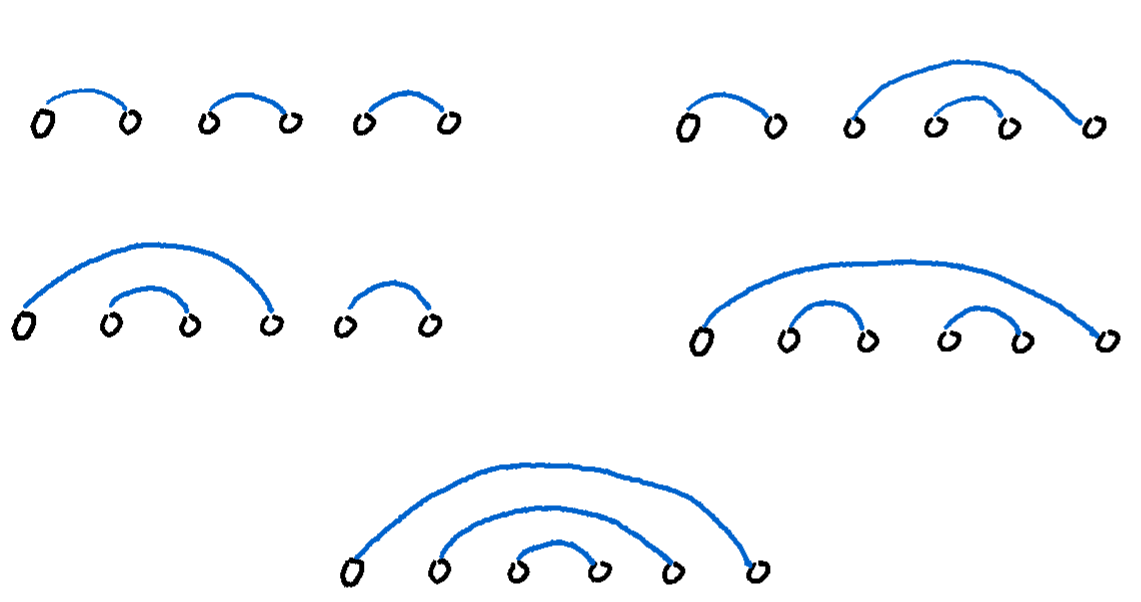
\includegraphics[width = 0.7\textwidth]{graphics/catalan_exercise_part1_figure.png}
  \caption{Fallet $n=3$ av fråga 4a.}
  \label{fig:q4a}
\end{figure}

Bevisa att $\ell_n$ är det $n$te Catalantalet.

\noindent
\textbf{Delfråga b:} \emph{(2.5p)}

Låt $b_n$ vara antalet sätt att rita $n+1$ punkter på en linje, hopkopplade med $n$ bågar, sådana att
\begin{itemize}
  \item bågarna inte passerar under linjen,
  \item bågarna inte skär varandra,
  \item grafen som bildas är ett träd,
  \item och i varje punkt går alla bågar ut åt samma håll.
\end{itemize}

Fallet då $n=3$ illustreras i Figur \ref{fig:q4b}. Bevisa att $b_n$ är det $n$te Catalantalet.\sidenote[][-0.7cm]{Ledtråd: Kan det någonsin inte finnas en båge mellan första och sista punkten?

Vad får du kvar om du tar bort den bågen?}

\begin{figure}
  \centering
  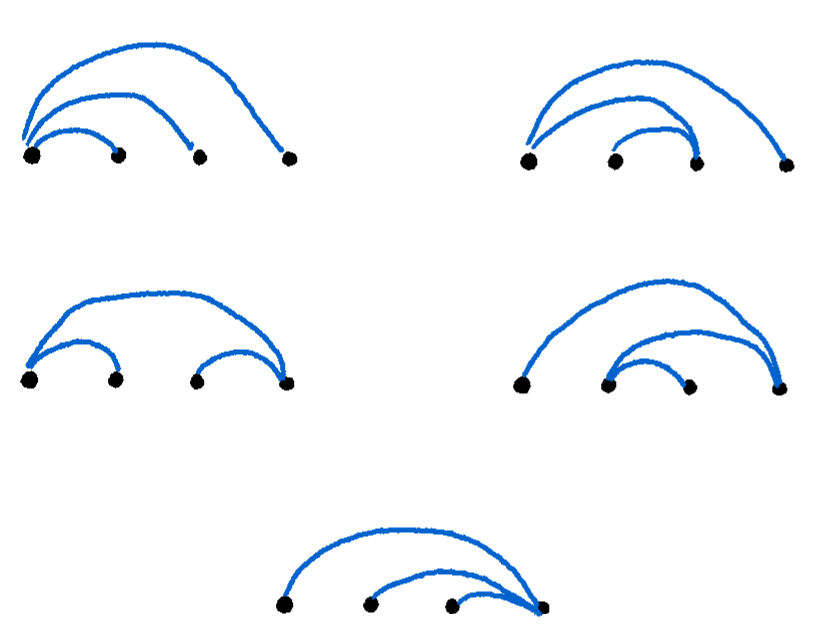
\includegraphics[width=0.7\textwidth]{graphics/catalan_exercise_part2_figure.png}
  \caption[][0.9cm]{Fallet $n=3$ av fråga 4b.}
  \label{fig:q4b}
\end{figure}



\section{Fråga 5 (5 poäng)} % intermezzo

I kursen bevisade vi följande proposition:

\begin{proposition}
  Antalet rotade ordnade binära oetiketterade träd som har $n-1$ interna noder ges av Catalantalen.
\end{proposition}

\textbf{Delfråga a:} \emph{3p}

Ge en definition för varje av termerna som dyker upp i det här påståendet.

\textbf{Delfråga b:} \emph{2p}

Bevisa propositionen.

\section{Fråga 6 (5 poäng)} % intermezzo

\textbf{Delfråga a:} \emph{(2p)} Hur finner man Prüferkoden för ett träd? Skriv Prüferkoden för trädet i Figur \ref{fig:prufer_code_tree}, och förklara hur du gick tillväga.

\begin{figure}
  \centering
  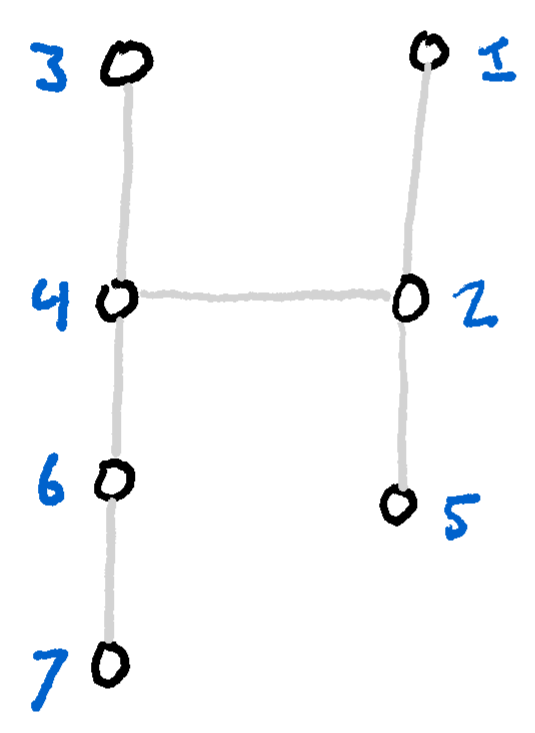
\includegraphics[width=0.4\textwidth]{graphics/prufer_code_tree.png}
  \caption{Ett träd med etiketter i blått, för vilket vi önskar finna Prüferkoden.}
  \label{fig:prufer_code_tree}
  % Prüferkoden är 24246
\end{figure}

\textbf{Delfråga b:} \emph{(3p)} Hur konstruerar man ett träd givet en Prüferkod? Rita trädet som motsvarar Prüferkoden
$$41377$$
och förklara hur du gick tillväga.

\section{Fråga 7 (5 poäng)} % del 3

När vi bevisade Caro-Weis sats så skapade vi oss en slumpmässig oberoende mängd genom att välja en slumpmässig permutation, på det sätt som illustreras i Figur \ref{fig:caro_wei}.

\begin{figure}
  \centering
  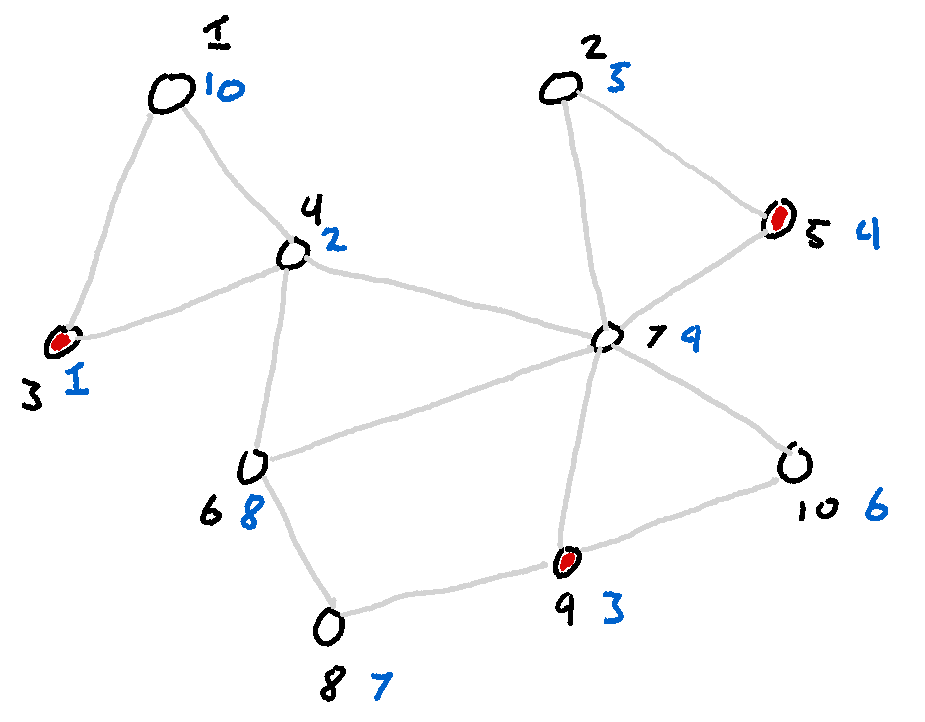
\includegraphics[width=0.8\textwidth]{graphics/Caro_Wei_construction.png}
  \caption{En figur, tagen ur föreläsningsanteckningarna, som illustrerar vårt bevis av Caro-Wei.}
  \label{fig:caro_wei}
\end{figure}

\textbf{Delfråga a:} \emph{(2p)} Beskriv hur vi konstruerade den oberoende mängden, och förklara varför denna konstruktion måste ge en oberoende mängd.

\textbf{Delfråga b:} \emph{(2p)} Beräkna väntevärdet av antalet noder i den oberoende mängden.

\textbf{Delfråga c:} \emph{(1p)} Formulera Caro-Weis sats, och använd vad vi gjort i de tidigare delarna av frågan för att bevisa den.

\section{Fråga 8 (5 poäng)} % del 3

\textbf{Delfråga a:} \emph{(2.5p)} En triangel i en graf är tre noder som har kanter mellan sig. Räkna ut väntevärdet av antalet trianglar i Erd\H{o}s-Renyi-grafen $G_{n,p}$.

\textbf{Delfråga b:} \emph{(2.5p)} Bevisa att om $p \leq n^{-(1+\epsilon)}$ för något $\epsilon > 0$ så finns det asymptotiskt nästan säkert inga trianglar i $G_{n,p}$.\sidenote[][]{Med ``asymptotiskt nästan säkert'' menar vi att sannolikheten att det finns en triangel går mot noll när $n$ går mot oändligheten.}

\pagebreak

\section{Formelsamling}

\section{Den tolvfaldiga vägen}

\begin{fullwidth}
  \begin{tabularx}{\linewidth}{l|ccc}
    & Lorem ipsum & dolor sit & amet consectetur\\
    \midrule
    adipiscing elit& \textcolor{red}{$x^n$} & \textcolor{red}{$\frac{x!}{(x-n)!}$} & \textcolor{red}{$x!\stirlingPart{n}{x}$} \\
    Suspendisse a nihil& \specialcell{\textcolor{red}{$\binom{n + x - 1}{n}$}} & {\textcolor{red}{$\binom{x}{n}$}} & \specialcell{$\binom{n - 1}{n - x}$} \\
    posuere etenim ergo& \specialcell{$\sum_{k=1}^{x} \stirlingPart{n}{k}$} & \specialcell{$1$ om $n \leq x$, $0$ annars} & \specialcell{\textcolor{red}{$\stirlingPart{n}{x}$}} \\
    ut non olivarum& \specialcell{$p_x(n + x)$} & \specialcell{$1$ om $n \leq x$, $0$ annars} & \specialcell{\textcolor{red}{$p_x(n)$}} 
  \end{tabularx}
\end{fullwidth}

\section{Räkneregler för genererande funktioner}

\begin{lemma}[Räkneregler för genererande funktioner]
  Antag att vi har en följd $\{a_k\}_{k=0}^\infty$, med genererande funktion $F_a$. Då gäller det att
    \begin{enumerate}
        \item För varje $j \geq 1$ är
        $$\sum_{k = j}^{\infty} a_k x^k = \left(\sum_{k=0}^{\infty}a_k x^k\right) - \left(\sum_{k=0}^{k=j-1} a_kx^k\right) = F_a(x) - \sum_{k=0}^{k=j-1} a_kx^k$$
        \item För alla $m \geq 0$, $l \geq -m$ gäller det att
        $$\sum_{k=m}^{\infty} a_k x^{k + l} = x^l\left(\sum_{k=m}^{\infty} a_k x^{k}\right) = x^l\left(F_a(x) - \sum_{k=0}^{m-1} a_k x^k\right)$$
        \item Det gäller att\sidenote[][]{Denna räkneregel kan förstås generealiseras till att högre potenser av $k$ motsvarar högre derivator -- och om vi istället delar med någon potens av $k$ får vi primitiva funktioner till den genererande funktionen.}
        $$\sum_{k=0}^{\infty} k a_k x^k = \frac{F_a'(x)}{x}.$$
    \end{enumerate}
\end{lemma}

\section{Vanliga genererande funktioner}

\begin{tabularx}{\linewidth}{cc}
  Följd & Genererande funktion\\
  \midrule
  $(1, 0, 0, \ldots)$ & $1$\\
  $(1,1,1,\ldots)$ & $\frac{1}{1-x}$\\
  $a_k = 1$ om $k \leq n$, $0$ annars & $\frac{1 - x^{n+1}}{1 - x}$\\
  Fixt $n$, $a_k = \binom{n}{k}$ & $(1+x)^n$\\
  Fixt $n$, $a_k = \binom{n+k-1}{k}$ & $\frac{1}{(1-x)^n}$\\
  \specialcell{Fibonaccitalen\\$f_0 = f_1 = 1$, $f_{k+1} = f_k + f_{k-1}$ för $k \geq 1$} & $\frac{1}{1 - x - x^2}$\\
  \specialcell{Indikatorfunktion för jämna talen\\$(1,0,1,0,1,0,\ldots)$} & $\frac{1}{1-x^2}$\\
  Catalantalen & $\frac{1 - \sqrt{1 - 4x}}{2x}$
\end{tabularx}

\begin{tabularx}{0.9\linewidth}{cc}
  Följd & Exponentiell genererande funktion\\
  \midrule
  $(1, 0, 0, \ldots)$ & $1$\\
  $(1, 1, 1, \ldots)$ & $e^x$\\
  $(0!, 1!, 2!, 3!, \ldots)$ & $\frac{1}{1-x}$\\
  Fixt $n$, $a_k = \frac{n!}{(n-k)!}$ & $(1 + x)^n$
\end{tabularx}

\section{Sannolikhetsteori}

\begin{lemma}
  Det gäller för alla händelser $A$ och $B$ att
  \begin{itemize}
      \item per definition är $\Prob{A} = \sum_{\omega \in A} \mu(\omega)$,
      \item så $\Prob{A^c} = 1 - \Prob{A}$,
      \item och om $A$ och $B$ har tomt snitt, $A\cap B = \emptyset$, så är $\Prob{A \cup B} = \Prob{A} + \Prob{B}$,
      \item och om de inte nödvändigtvis har tomt snitt har vi att
      $$\Prob{A \cup B} = \Prob{A} + \Prob{B} - \Prob{A \cap B}.$$
      \item $\Prob{A \cap B} = \Prob{A \given B}\Prob{B}$,
      \item och per definition är $A$ och $B$ oberoende precis när $\Prob{A \cap B} = \Prob{A}\Prob{B}$.
  \end{itemize}
\end{lemma}

\begin{lemma}
  Om $(\Omega, \mu)$ är något sannolikhetsrum, $A \subseteq \Omega$ någon händelse, och $X, Y: \Omega \to \R$ samt $Z: \Omega \to V$ är slumpvariabler som tar värden i $\R$ och i någon godtycklig mängd $V$, så gäller att:
  \begin{enumerate}
      \item $$\E{X} = \sum_{x \in X(\Omega)} x \Prob{X = x} = \sum_{\omega \in \Omega} X(\omega)\mu(\omega).$$
      \item För alla $a, b \in \R$ så är
      $$\E{aX + bY} = a\E{X} + b\E{Y}.$$
      Väntevärdet är alltså en linjär funktional.
      \item $$\Prob{A} = \E{\indSet{A}}.$$
      \item Om $X(\omega) \leq C$ för varje $\omega$, eller ekvivalent om $\Prob{X \leq C} = 1$, så är $\E{X} \leq C$.
      \item Om $\E{X} = C$ så finns det åtminstone ett $\omega$ sådant att $X(\omega) \geq C$.
      \item Om $Z$ är likformigt fördelad på $V$ så gäller det för varje delmängd $W \subseteq V$ att
      $$\Prob{Z \in W} = \frac{\abs{W}}{\abs{V}}.$$
  \end{enumerate}
\end{lemma}


%\bibliography{references}
%\bibliographystyle{plainnat}

\end{document}
